\documentclass[aspectratio=169,10pt]{beamer}
\usetheme{Madrid}
\usecolortheme{default}
\usepackage{tikz}
\usepackage{booktabs}
\usepackage{fontawesome5}
\usepackage{xcolor}
\usepackage{amsmath}
\usetikzlibrary{arrows.meta,shadows,positioning,fit,shapes.geometric}

% ── palette ──────────────────────────────────────────────────────────
\definecolor{c1}{RGB}{41,128,185}
\definecolor{c2}{RGB}{52,152,219}
\definecolor{c3}{RGB}{155,89,182}
\definecolor{c4}{RGB}{142,68,173}
\definecolor{c5}{RGB}{230,126,34}
\definecolor{c6}{RGB}{211,84,0}
\definecolor{hit}{RGB}{39,174,96}
\definecolor{miss}{RGB}{192,57,43}
\definecolor{warn}{RGB}{243,156,18}

\setbeamercolor{frametitle}{bg=c1,fg=white}
\setbeamercolor{title}{fg=white}
\setbeamercolor{structure}{fg=c1}
\setbeamertemplate{navigation symbols}{}
\setbeamertemplate{footline}[frame number]
\setbeamerfont{frametitle}{series=\bfseries}

\title{\textbf{graph-rag}\\[4pt]
       \large CPG-Based Vulnerability Retrieval}
\subtitle{Master's Thesis — Technical Progress}
\author{Lívia}
\institute{TU Munich · Siemens AI Engineering}
\date{\today}

\begin{document}

% ── title ─────────────────────────────────────────────────────────────
\begin{frame}
\titlepage
\end{frame}

% ── outline ───────────────────────────────────────────────────────────
% \begin{frame}{Agenda}
% \tableofcontents
% \end{frame}

\section{Motivation}
\section{System Architecture}
\section{Data Foundation}
\section{Graph Representation}
\section{Embedders}
\section{RAG Backends}
\section{Experiments \& Early Results}
\section{Next Steps}

% ══════════════════════════════════════════════════════════════════════
\section{Motivation}
% ══════════════════════════════════════════════════════════════════════

\begin{frame}{Why Graph-Based Vulnerability Retrieval?}
\begin{columns}[T]
\begin{column}{0.55\textwidth}
  \textbf{The problem:} Given a new vulnerable function, find the
  most structurally similar historical CVEs — enabling automated
  patch suggestion.

  % \vspace{1em}
  % \begin{block}{Why not text search?}
  %   Two buffer overflows in different codebases share \emph{structure},
  %   not tokens. Variable names, formatting, and language style vary;
  %   the \emph{program dependence pattern} does not.
  % \end{block}

  \vspace{0.8em}
  \textbf{Key insight:} Code Property Graphs (CPGs) unify AST,
  CFG, and PDG into one representation —
  the \emph{diff} between vulnerable and patched CPG isolates
  exactly what changed.
\end{column}
\begin{column}{0.42\textwidth}
  \centering
  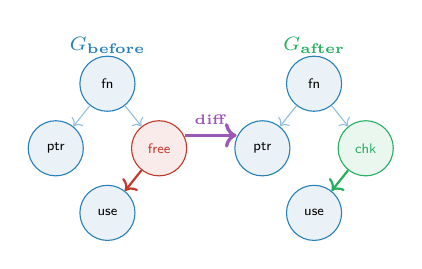
\begin{tikzpicture}[scale=0.82,
    node/.style={circle,draw=c1,fill=c1!10,minimum size=0.7cm,
                 font=\tiny\sffamily,inner sep=1pt},
    rnode/.style={circle,draw=miss,fill=miss!10,minimum size=0.7cm,
                  font=\tiny\sffamily,inner sep=1pt},
    gnode/.style={circle,draw=hit,fill=hit!10,minimum size=0.7cm,
                  font=\tiny\sffamily,inner sep=1pt}]
    % before graph
    \node[font=\scriptsize\bfseries,c1] at (0,2.6) {$G_{\text{before}}$};
    \node[node]  (a) at (0,2)    {fn};
    \node[node]  (b) at (-0.8,1) {ptr};
    \node[rnode] (c) at (0.8,1)  {\textcolor{miss}{free}};
    \node[node]  (d) at (0,0)    {use};
    \draw[->,c1!50] (a)--(b); \draw[->,c1!50] (a)--(c);
    \draw[->,miss,thick] (c)--(d);
    % after graph
    \node[font=\scriptsize\bfseries,hit] at (3.2,2.6) {$G_{\text{after}}$};
    \node[node]  (a2) at (3.2,2)   {fn};
    \node[node]  (b2) at (2.4,1)   {ptr};
    \node[gnode] (c2) at (4.0,1)   {\textcolor{hit}{chk}};
    \node[node]  (d2) at (3.2,0)   {use};
    \draw[->,c1!50] (a2)--(b2); \draw[->,c1!50] (a2)--(c2);
    \draw[->,hit,thick] (c2)--(d2);
    % diff arrow
    \draw[->,very thick,c3] (1.2,1.2) -- node[above,font=\tiny,c3]
      {\textbf{diff}} (2.0,1.2);
  \end{tikzpicture}

  \vspace{0.5em}
  {\scriptsize\color{gray} Changed node (red→green) isolated by semantic diff}
\end{column}
\end{columns}
\end{frame}

% ══════════════════════════════════════════════════════════════════════
\section{System Architecture}
% ══════════════════════════════════════════════════════════════════════

\begin{frame}{System Architecture: End-to-End Pipeline}
\centering
\resizebox{\textwidth}{!}{%

\begin{tikzpicture}[node distance=0pt,
  block/.style={rectangle,minimum width=3.2cm,minimum height=1.4cm,
                text centered,text width=2.9cm,draw=white,line width=1.5pt,
                font=\sffamily\small\bfseries,rounded corners=3pt}]

  \node (n1) [block,fill=c1,text=white]
    {I.\\Ingestion \&\\Sanitisation};
  \node (n2) [block,fill=c2,text=white,right=0.5cm of n1]
    {II.\\CPG\\Construction};
  \node (n3) [block,fill=c3,text=white,right=0.5cm of n2]
    {III.\\Vulnerability\\Diff};
  \node (n4) [block,fill=c4,text=white,right=0.5cm of n3]
    {IV.\\Graph\\Embedding};
  \node (n5) [block,fill=c5,text=white,right=0.5cm of n4]
    {V.\\Vector\\Index};
  \node (n6) [block,fill=c6,text=white,right=0.5cm of n5]
    {VI.\\Agentic\\Synthesis};

  % chevron connectors
  \foreach \i [evaluate=\i as \next using int(\i+1)] in {1,2,3,4,5}{
    \fill[white!30] (n\i.north east) -- ++(0.4,-0.7) -- (n\i.south east)--cycle;
  }

  % sub-labels
  \foreach \n/\lbl in {n1/C\,/\,C++ Source,
                        n2/Joern CPG,
                        n3/$G_{\text{vuln}}$ subgraph,
                        n4/128-d vector,
                        n5/FAISS\,/\,HNSW,
                        n6/Patch Agents}{
    \node[below=0.15cm of \n,font=\tiny\sffamily\color{black!55}] {\lbl};
  }
\end{tikzpicture}}

\vfill
\begin{columns}[t]
  \begin{column}{0.33\textwidth}\centering
    \textbf{\textcolor{c1}{Data Layer}}\\
    \scriptsize Dataset interface to CPG format.
  \end{column}
  \begin{column}{0.33\textwidth}\centering
    \textbf{\textcolor{c3}{Vector Layer}}\\
    \scriptsize Structural diff $\rightarrow$ latent space projection.
  \end{column}
  \begin{column}{0.33\textwidth}\centering
    \textbf{\textcolor{c5}{Agent Layer}}\\
    \scriptsize LLM reasoning augmented with retrieved CVE context.
  \end{column}
\end{columns}
\end{frame}

% ══════════════════════════════════════════════════════════════════════
\section{Data Foundation}
% ══════════════════════════════════════════════════════════════════════

\begin{frame}{Data Foundation: Datasets \& Loader Design}
\begin{columns}[T]
\begin{column}{0.52\textwidth}
  \textbf{Supported datasets} — all yield \texttt{FunctionPair}
  objects via a common \texttt{BaseDataset} interface:

  \vspace{0.6em}
  \begin{description}[\textbf{CVEFixes}]
    \item[\textbf{AutoPatch}] Folder-per-CVE with original source
      \emph{and} LLM-reimplemented variants
      (GPT-4o, DeepSeek-R1, LLaMA, o3-mini).
      Enables augmented generalisation testing.
      % \item[\textbf{BigVul}] 3,500+ CVEs as CSV with
      % \texttt{func\_before}/\texttt{func\_after} columns.
      % Largest C/C++ vulnerability dataset.
    \item[\textbf{CVEFixes} (Optional)] SQLite DB; method-level before/after
      pairs linked to commit history.
  \end{description}

  % \vspace{0.6em}
  
\end{column}
\begin{column}{0.45\textwidth}
  \begin{block}{Design decision}
    \texttt{export\_jobs()} parallelises Joern over functions;
    \texttt{stream()} feeds the index builder.
    Adding a new dataset = one class, two methods.
  \end{block}
  % \centering
  % \begin{tikzpicture}[scale=0.9,
  %   ds/.style={rounded corners=4pt,draw=c1!50,fill=c1!8,
  %              minimum width=3.2cm,minimum height=0.65cm,
  %              font=\scriptsize\sffamily,align=center},
  %   iface/.style={rounded corners=4pt,draw=c3,fill=c3!10,
  %                 minimum width=3.2cm,minimum height=0.65cm,
  %                 font=\scriptsize\sffamily\bfseries,align=center},
  %   out/.style={rounded corners=4pt,draw=hit,fill=hit!8,
  %               minimum width=3.2cm,minimum height=0.65cm,
  %               font=\scriptsize\sffamily,align=center}]
  %   \node[ds] (bv) at (0,3.2)  {BigVul (CSV)};
  %   \node[ds] (cf) at (0,2.4)  {CVEFixes (SQLite)};
  %   \node[ds] (ap) at (0,1.6)  {AutoPatch (folders)};
  %   \node[iface] (bd) at (0,0.7) {BaseDataset interface};
  %   \draw[->,c1!60] (bv)--(bd);
  %   \draw[->,c1!60] (cf)--(bd);
  %   \draw[->,c1!60] (ap)--(bd);
  %   % \draw[->,c3,thick] (bd)--(fp);
  % \end{tikzpicture}
\end{column}
\end{columns}
\end{frame}

% ══════════════════════════════════════════════════════════════════════
\section{Graph Representation}
% ══════════════════════════════════════════════════════════════════════

\begin{frame}{From Source Code to Vulnerability Subgraph}
\begin{columns}[T]
\begin{column}{0.52\textwidth}

  \textbf{Step 1 — CPG Export (Joern)}\\[2pt]
  \texttt{joern-export --repr all} produces one
  \texttt{export.xml} per function covering
  AST, CFG, and PDG edges.

  \vspace{0.8em}
  \textbf{Step 2 — Graph Diff}\\[2pt]
  Match nodes by Joern ID.
  \textit{Identified problem:} Joern assigns non-deterministic IDs across runs — ID-based
  diff produced $G_{\text{vuln}} \approx G_{\text{before}}$,
  making all graphs indistinguishable.

  % \vspace{0.6em}
  % Changed nodes are typed and weighted:

  % \vspace{0.3em}
  % \begin{tabular}{ll}
  %   \texttt{removed} / \texttt{added} & weight 1.0 \\
  %   \texttt{mutated} (code changed)   & weight 0.8 \\
  %   \texttt{rewired} (edge changed)   & weight 0.6 \\
  %   \texttt{context} ($n$-hop)        & weight 0.1--0.3 \\
  % \end{tabular}

  \vspace{0.6em}
  \textbf{Step 3 — CPG Slice}\\[2pt]
  Extract the nodes that diverge and its neighbors with a hop-based of 1 scheme.
  % \textbf{Step 3 — PDG-Anchored Slice}\\[2pt]

  % Neighbourhood expansion follows only \texttt{CFG},
  % \texttt{CDG}, \texttt{REACHING\_DEF} edges —
  % eliminating the AST-dominated noise that
  % inflates $G_{\text{vuln}}$.

\end{column}
\begin{column}{0.3\textwidth}
  \centering
  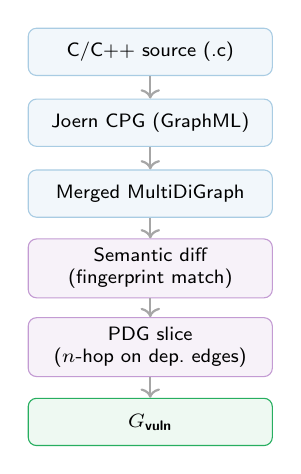
\begin{tikzpicture}[
    box/.style={draw=c1!40,rounded corners=3pt,fill=c1!6,
                minimum width=3.1cm,minimum height=0.6cm,
                font=\scriptsize\sffamily,align=center},
    dec/.style={draw=c3!60,rounded corners=3pt,fill=c3!8,
                minimum width=3.1cm,minimum height=0.6cm,
                font=\scriptsize\sffamily,align=center},
    res/.style={draw=hit,rounded corners=3pt,fill=hit!8,
                minimum width=3.1cm,minimum height=0.6cm,
                font=\scriptsize\sffamily\bfseries,align=center}]
    \node[box] (s)  at (0, 4.5) {C/C++ source (.c)};
    \node[box] (j)  at (0, 3.6) {Joern CPG (GraphML)};
    \node[box] (m)  at (0, 2.7) {Merged MultiDiGraph};
    \node[dec] (d)  at (0, 1.75) {Semantic diff\\(fingerprint match)};
    \node[dec] (sl) at (0, 0.75) {PDG slice\\($n$-hop on dep.\ edges)};
    \node[res] (gv) at (0, -0.20) {$G_{\text{vuln}}$};
    \foreach \a/\b in {s/j,j/m,m/d,d/sl,sl/gv}
      \draw[->,thick,black!35] (\a)--(\b);
  \end{tikzpicture}
\end{column}
\end{columns}
\end{frame}

% \begin{frame}{Graph Extraction Strategies Compared}
% \centering
% \begin{tabular}{lp{5.8cm}cc}
%   \toprule
%   \textbf{Strategy} & \textbf{Rationale} & \textbf{Signal} & \textbf{Noise} \\
%   \midrule
%   ID-based diff & Original approach; broken by non-det.\ IDs
%     & \textcolor{miss}{\faIcon{times}} & \textcolor{miss}{\faIcon{times}} \\[3pt]
%   Semantic $n$-hop & Fingerprint matching + context ($n{=}1,2$ optimal)
%     & \textcolor{warn}{\faIcon{adjust}} & \textcolor{warn}{\faIcon{adjust}} \\[3pt]
%   CFG-only & Removes AST dominance; focuses on execution paths
%     & \textcolor{warn}{\faIcon{adjust}} & \textcolor{hit}{\faIcon{check}} \\[3pt]
%   PDG slice & Bidirectional BFS on \texttt{REACHING\_DEF}+\texttt{CDG};
%     captures data \& control deps
%     & \textcolor{hit}{\faIcon{check}} & \textcolor{hit}{\faIcon{check}} \\[3pt]
%   Motif histogram & 8-dim count of vulnerability-shaped 3-node patterns;
%     CWE-agnostic
%     & \textcolor{hit}{\faIcon{check}} & \textcolor{hit}{\faIcon{check}} \\
%   \bottomrule
% \end{tabular}

% \vspace{1em}
% \begin{block}{Key finding}
%   AST edges represent $> 70\%$ of CPG edges in most exports.
%   Strategies that restrict to PDG/CFG reduce $|G_{\text{vuln}}|$ and
%   increase signal density — fewer nodes, more vulnerability-relevant.
% \end{block}
% \end{frame}

% ══════════════════════════════════════════════════════════════════════
\section{Embedders}
% ══════════════════════════════════════════════════════════════════════

\begin{frame}{Unsupervised Graph Embedders}
\textit{All embedders require no labelled training data.
Output: L2-normalised 128-dim vector per function graph.}

\vspace{0.5em}
\begin{columns}[T]
\begin{column}{0.48\textwidth}

  \textbf{\textcolor{c1}{Structural embedders}}
  \begin{description}[\textbf{Combined}]
    \item[\textbf{NetLSD}] Heat trace of the graph Laplacian.
      Permutation-invariant; captures global shape.
      \textit{Collapses on graphs $<5$ nodes.}
    \item[\textbf{WL}] Weisfeiler-Lehman colour refinement. Subtree kernel equivalent.
    \item[\textbf{GIN}] 3-layer Graph Isomorphism Network with
      frozen random weights. Johnson-Lindenstrauss
      distance preservation via MLP non-linearity.
    \item[\textbf{Combined}] NetLSD + WL + GIN concatenated.
    More robust to individual collapse.
  \end{description}

\end{column}
% \begin{column}{0.48\textwidth}

%   \textbf{\textcolor{c3}{Semantic embedder}}
%   \begin{description}[\textbf{Motif}]
%     \item[\textbf{Motif}] Three signals concatenated:
%       \begin{itemize}
%         \item Motif histogram (8-dim vulnerability patterns)
%         \item CODE token features: ptr / alloc / free / lock / cast
%           density per graph
%         \item NetLSD on PDG slice (16-dim)
%       \end{itemize}
%       Projected via Gaussian random projection.
%       \textit{Designed for CWEs where topology is uniform.}
%   \end{description}

%   \vspace{0.8em}
%   \begin{block}{\texttt{diff\_weight} bias}
%     All embedders weight pooling toward \texttt{removed},
%     \texttt{added}, and \texttt{mutated} nodes — ensuring
%     changed code dominates the embedding.
%   \end{block}
% \end{column}
\end{columns}
\end{frame}

% ══════════════════════════════════════════════════════════════════════
\section{RAG Backends}
% ══════════════════════════════════════════════════════════════════════

\begin{frame}{RAG Index Backends}
Two interchangeable backends — identical \texttt{add / save / load}
interface, swap via \texttt{config.yaml}.

\vspace{0.8em}
\begin{columns}[T]
\begin{column}{0.46\textwidth}
  \begin{block}{FAISS Flat (IndexFlatIP)}
    \begin{itemize}
      \item Exact cosine search (inner product on L2-normed vectors)
      \item Guaranteed correct top-$k$
      \item Linear $O(n)$ query — suitable up to $\sim$100k vectors
      \item \textbf{Role:} correctness baseline in all experiments
    \end{itemize}
  \end{block}
\end{column}
\begin{column}{0.46\textwidth}
  \begin{block}{HNSW}
    \begin{itemize}
      \item Approximate nearest-neighbour via proximity graph
      \item $O(\log n)$ query time
      \item Tunable recall/speed: \texttt{M} (connectivity),
        \texttt{ef\_search} (beam width)
      \item \textbf{Role:} production backend at $>$10k vectors
    \end{itemize}
  \end{block}
\end{column}
\end{columns}

\vspace{1em}
\centering
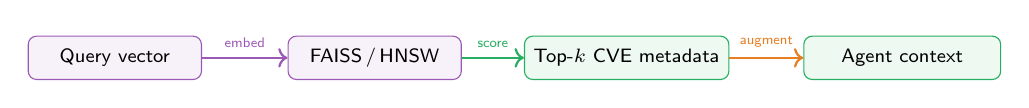
\begin{tikzpicture}[
  q/.style={rounded corners=3pt,draw=c3,fill=c3!8,
            minimum width=2.2cm,minimum height=0.55cm,
            font=\scriptsize\sffamily,align=center},
  r/.style={rounded corners=3pt,draw=hit,fill=hit!8,
            minimum width=2.5cm,minimum height=0.55cm,
            font=\scriptsize\sffamily,align=center}]
  \node[q] (qv) at (0,0)    {Query vector};
  \node[q] (fi) at (3.3,0)  {FAISS\,/\,HNSW};
  \node[r] (tk) at (6.5,0)  {Top-$k$ CVE metadata};
  \node[r] (ag) at (10,0)  {Agent context};
  \draw[->,thick,c3]  (qv)--(fi)
    node[midway,above,font=\tiny\sffamily] {embed};
  \draw[->,thick,hit] (fi)--(tk)
    node[midway,above,font=\tiny\sffamily] {score};
  \draw[->,thick,c5]  (tk)--(ag)
    node[midway,above,font=\tiny\sffamily] {augment};
\end{tikzpicture}
\end{frame}

% ══════════════════════════════════════════════════════════════════════
\section{Experiments \& Early Results}
% ══════════════════════════════════════════════════════════════════════

\begin{frame}{Experiment Design}
\begin{columns}[T]
\begin{column}{0.50\textwidth}
  \textbf{Grid evaluated:}
  $\text{embedder} \times \text{backend} \times \text{graph variant}$

  \vspace{0.5em}
  \textbf{Metrics} (all unsupervised — no labelled queries yet):
  \begin{description}[\textbf{CWE recall}]
    \item[\textbf{Hit@K}] Fraction of queries where correct CVE
      appears in top-$K$ ($K \in \{1,5,10\}$).
    \item[\textbf{MRR}] Mean reciprocal rank.
    \item[\textbf{CWE recall}] Fraction of top-$K$ sharing
      the query's CWE type — measures cluster quality.
    \item[\textbf{Eff. dim}] Participation ratio of PCA
      eigenvalues — detects embedding collapse.
  \end{description}

\end{column}
\begin{column}{0.47\textwidth}
  \centering
  % radar-like bar showing metric coverage
  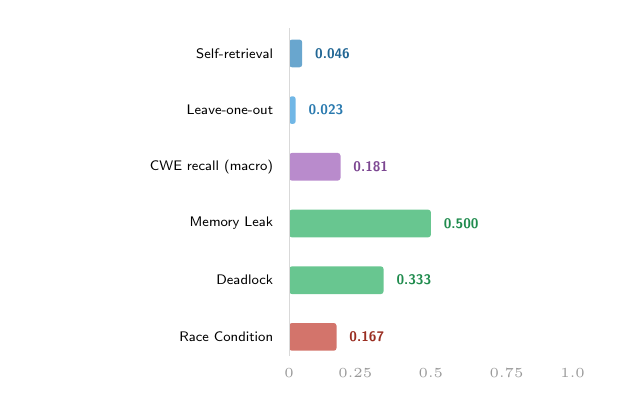
\begin{tikzpicture}[scale=0.8]
    \foreach \y/\lbl/\col/\val in {
      4.5/{Self-retrieval}/c1/0.046,
      3.6/{Leave-one-out}/c2/0.023,
      2.7/{CWE recall (macro)}/c3/0.181,
      1.8/{Memory Leak}/hit/0.500,
      0.9/{Deadlock}/hit/0.333,
      0.0/{Race Condition}/miss/0.167}{
      \node[left,font=\tiny\sffamily,text width=3cm,align=right]
        at (0,\y) {\lbl};
      \fill[\col!70,rounded corners=1pt]
        (0.1,\y-0.22) rectangle ({0.1+4.5*\val},\y+0.22);
      \node[right,font=\tiny\sffamily\bfseries,\col!80!black]
        at ({0.1+4.5*\val+0.05},\y) {\val};
    }
    \draw[black!15] (0.1,-0.3)--(0.1,4.9);
    \foreach \x/\v in {0.1/0, 1.15/0.25, 2.35/0.5, 3.55/0.75, 4.6/1.0}
      \node[below,font=\tiny\color{black!40}] at (\x,-0.35) {\v};
  \end{tikzpicture}

  {\scriptsize\color{gray} Best result: NetLSD on $G_{\text{vuln}}$, 65 pairs}
\end{column}
\end{columns}
\end{frame}

\begin{frame}{Key Findings}
\begin{enumerate}
  \item[\faIcon{bug}\;] \textbf{ID-based diff was fatally flawed.}
    Joern IDs are non-deterministic across runs.
    $G_{\text{vuln}} \approx G_{\text{before}}$ made all graphs
    structurally indistinct.
    \textit{Fix: fingerprint matching by \texttt{(type, CODE)}.}

  \vspace{0.5em}
  \item[\faIcon{compress-arrows-alt}\;]
    \textbf{Embedding space collapsed.}
    Effective dimension $\approx 1$; pairwise cosine $> 0.999$.
    Causes: shared scaffold boilerplate nodes injected by wrapper,
    AST-edge dominance ($> 70\%$ of edges), and NetLSD/WL collapse
    on small graphs.
    \textit{Fix: PDG-anchored slicing + scaffold node removal.}

  \vspace{0.5em}
  \item[\faIcon{chart-bar}\;] \textbf{CWE retrieval is structurally determined.}
    CWEs whose patches \emph{add or remove nodes}
    (Memory Leak, Deadlock) retrieve well.
    CWEs whose patches change \emph{ordering or pointer state}
    (UAF, Race Condition) are near-undetectable by topology alone.

  \vspace{0.5em}
  \item[\faIcon{code}\;] \textbf{Semantic features are necessary.}
    t-SNE of node-type histograms shows random CWE distribution —
    topology does not separate vulnerability classes.
    CODE attribute coverage is 100\%: semantic embedders have
    the raw material to work with.
    \textit{Motif embedder and PDG-slice experiments pending.}
\end{enumerate}
\end{frame}

\begin{frame}{CWE-Level Retrieval — Current State}
\centering
\vspace{-0.3em}

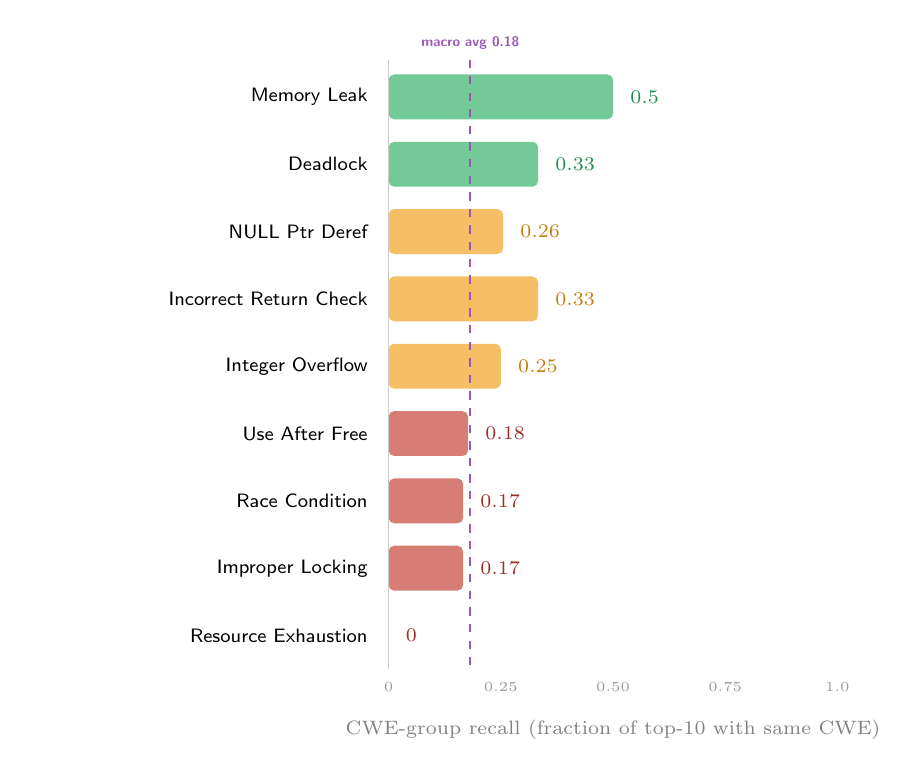
\begin{tikzpicture}[scale=0.95]
  % y-axis labels and bars
  \foreach \y/\cwe/\val/\col in {
    7.2/{Memory Leak}/0.50/hit,
    6.3/{Deadlock}/0.333/hit,
    5.4/{NULL Ptr Deref}/0.255/warn,
    4.5/{Incorrect Return Check}/0.333/warn,
    3.6/{Integer Overflow}/0.25/warn,
    2.7/{Use After Free}/0.177/miss,
    1.8/{Race Condition}/0.166/miss,
    0.9/{Improper Locking}/0.166/miss,
    0.0/{Resource Exhaustion}/0.0/miss}{
    \node[left,font=\scriptsize\sffamily,text width=4.2cm,align=right]
      at (0,\y) {\cwe};
    \fill[\col!65,rounded corners=2pt]
      (0.15,\y-0.3) rectangle ({0.15+6.0*\val},\y+0.3);
    \node[right,font=\scriptsize\sffamily\bfseries,\col!80!black]
      at ({0.15+6.0*\val+0.1},\y) {\pgfmathprintnumber[fixed,precision=2]{\val}};
  }

  % macro avg line
  \draw[c3,thick,dashed] ({0.15+6.0*0.1819},-0.4)--({0.15+6.0*0.1819},7.7)
    node[above,font=\tiny\sffamily\bfseries,c3] {macro avg 0.18};

  % axis
  \draw[black!20] (0.15,-0.45)--(0.15,7.7);
  \foreach \x/\v in {0.15/0, 1.65/0.25, 3.15/0.50, 4.65/0.75, 6.15/1.0}
    \node[below,font=\tiny\color{black!40}] at (\x,-0.5) {\v};
  \node[below,font=\scriptsize\color{black!50}] at (3.15,-1.0)
    {CWE-group recall (fraction of top-10 with same CWE)};
\end{tikzpicture}

\vspace{0.2em}
{\scriptsize
  \textcolor{hit}{\faIcon{circle}}\;Structurally distinctive \quad
  \textcolor{warn}{\faIcon{circle}}\;Moderate \quad
  \textcolor{miss}{\faIcon{circle}}\;Topology insufficient — semantic features needed
}
\end{frame}

% ══════════════════════════════════════════════════════════════════════
\section{Next Steps}
% ══════════════════════════════════════════════════════════════════════

\begin{frame}{Next Steps}
\begin{columns}[T]
\begin{column}{0.48\textwidth}
  % \textbf{Immediate (in progress)}
  % \begin{enumerate}
  %   \item Validate PDG edge export — confirm
  %     \texttt{REACHING\_DEF} density before
  %     investing in PDG-slice experiments.
  %   \item Run E7/E8: motif embedder on PDG slice
  %     vs.\ pure semantic baseline.
   
  % \end{enumerate}

  \vspace{0.8em}
  \textbf{Short term}
  \begin{enumerate}\setcounter{enumi}{3}
    \item Construct held-out query set with known
      CVE targets for honest precision/recall.
    
    \item Change the calculation of graph differences. 
      Instead of using the graph difference sets, look for a semantic difference (change of the nodes contents).
     \item Fix scaffold contamination — annotate
      and exclude boilerplate Joern nodes.
  \end{enumerate}
\end{column}
\begin{column}{0.3\textwidth}
  % \textbf{Research questions open}
  % \begin{enumerate}\setcounter{enumi}{6}
  %   \item \textbf{RQ1:} Does PDG-anchored embedding
  %     outperform spectral embedding for
  %     data-dependency CWEs (UAF, race)?
  %   \item \textbf{RQ2:} Does motif histogram alone
  %     outperform NetLSD?
  %     (If yes: topology adds noise, not signal.)
  %   \item \textbf{RQ3:} Can the system generalise
  %     to CVEs unseen during indexing?
  %     (Temporal split: train pre-$Y$, query $Y{+}1$.)
  %   \item \textbf{RQ4:} What is the minimum index
  %     size for clinically useful precision@5?
  % \end{enumerate}

  \vspace{0.5em}
  \begin{block}{Current Goal}
    Find a sweetspot of the graph content and diff operation to then focus on $G_{\text{vuln}}$
    semantic embedder, then iterate.
  \end{block}
\end{column}
\end{columns}
\end{frame}

\begin{frame}[plain]
\centering
\vspace{3em}
% {\Large\bfseries\color{c1} Thank you}\\[1em]
% {\color{gray} Questions welcome}\\[2em]
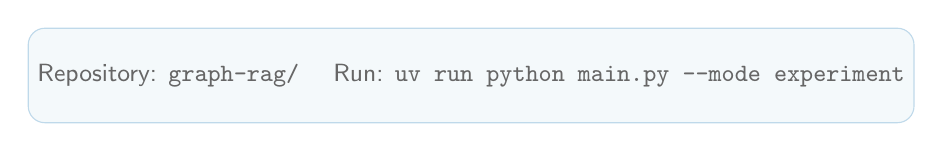
\begin{tikzpicture}
  \node[draw=c1!30,rounded corners=6pt,fill=c1!5,
        minimum width=8cm,minimum height=1.2cm,
        font=\small\sffamily\color{black!60},align=center]
    {Repository: \texttt{graph-rag/} \quad
     Run: \texttt{uv run python main.py --mode experiment}};
\end{tikzpicture}
\end{frame}

\end{document}